%!Mode:: "TeX:UTF-8"
\documentclass[a4paper,12pts]{article}

\usepackage[polish]{babel}
\usepackage[utf8]{inputenc}
\usepackage{fontspec}
\setmainfont{Calibri}

\linespread{1.15}

\usepackage{caption}
\captionsetup{%
	font={footnotesize},
	labelfont={bf}
}

\usepackage{anysize}
\usepackage{geometry}

\usepackage{graphicx}

% Plik szablonowy do wykorzystania pózniej - nie zmieniaj go!

\begin{document}
	\thispagestyle{empty}
	\begin{flushleft}
		Wydział Elektrotechniki, Automatyki, Informatyki i Inżynierii Biomedycznej \\
		Informatyka, rok II \\
		Zespół numer 3 \\
		Piotr Kucharski \\
		Dominik Zabłotny \\
		\vspace*{\fill}
		%-----------NUMER CWICZENIA--------%
		{\large \textbf{Sprawozdanie z ćwiczenia nr 32} } \\
		%-----------TEMAT ĆWICZENIA--------%
		Mostek Wheatstone'a		
		\vfill	
		%-----------DATA-------------%
		25 października 2017r
	\end{flushleft}
	
	\newpage
	
%--------------------------------------------------------------------------------------------------------------
	
	\section{Wstęp}
	
	\subsection{Cele ćwiczenia}
	
	Celem wykonywanego ćwiczenia jest praktyczne zastosowanie prawa Kirchhoffa oraz sprawdzenie zależności określających opór zastępczy dla połączeń szeregowych i równoległych.
	
%--------------------------------------------------------------------------------------------------------------
	
	\subsection{Wprowadzienie teoretyczne}
	
	\subsubsection{Pierwsze Prawo Kirchhoffa}
	
	\textit{Twierdzenie o punkcie rozgałęzienia.} Algebraiczna suma natężeń prądów przepływających przez punkt rozgałęzienia (węzeł) jest równa zeru:
	
	\begin{equation}
		\sum_{i=1}^{n} I_{i} = 0
	\end{equation}
	
	Twierdzenie o punkcie rozgałęzienia wynika z zasady zachowana ładunku.
	
%--------------------------------------------------------------------------------------------------------------	
	
	\subsubsection{Drugie Prawo Kirchhoffa}
	
	\textit{Twierdzenie o obwodzie zamkniętym.} Algebraiczna suma sił elektromotorycznych i przyrostów napięć na dowolnym obwodzie zamkniętym jest równa zeru (spadek napięcia jest przyrostem ujemnym napięcia):
	
	\begin{equation}
		\sum_{i=1}^{n} \varepsilon_{i} + \sum_{i=1}^{m} I_{i} R_{i} = 0
	\end{equation}
	
	Twierdzenie o obwodzie zamkniętym wynika z zasady zachowania energii.
	
%--------------------------------------------------------------------------------------------------------------	

	\subsubsection{Opór elektryczny}
	
	Opór elektryczny $R$ (\textit{Rezystancja}) to wielkość charakteryzująca relacje między napięciem a natężeniem prądu elektrycznego w obwodach prądu stałego. Najczęściej mówi się, że opór elektryczny jest to zdolność materiału do przewodzenia prądu, który definiujemy wzorem:
	
	\begin{equation}
		R = \frac{U}{I} \textrm{ [$\Omega$]}
	\end{equation}

	gdzie:
	\begin{itemize}
		\item $R$ ~-- opór elektryczny [$\Omega$]
		\item $U$ ~-- napięcie prądu [V]
		\item $I$ ~-- natężenie prądu [A]
	\end{itemize}

%--------------------------------------------------------------------------------------------------------------
	
	\subsubsection{Opór właściwy}
	
	Opór właściwy $\rho$ (\textit{Rezystowność}) to wielkość charakteryzująca materiały pod względem przewodnictwa elektrycznego. Określana jako trudność na jaką jaką natrafiają przemieszczające się elektrony. Opór właściwy zależy od długości przewodu, jego przekroju poprzecznego oraz materiału z jakiego został wykonany. Rezystowność definiujemy wzorem:
	
	\begin{equation}
		\rho = \frac{R \cdot S}{l} \textrm{  [$\Omega \cdot$ \textrm{m}]}
	\end{equation}

	gdzie: 
	\begin{itemize}
		\item $\rho$ ~-- opór właściwy [$\Omega \cdot \textrm{m}$]
		\item $R$ ~-- opór elektryczny [$\frac{\textrm{kg} \cdot \frac{\textrm{m}^{2}}{\textrm{s}^{2}}}{\textrm{A} \cdot \textrm{s}}$]
		\item $S$ ~-- pole przekroju poprzecznego [\textrm{m}$^{2}$]
		\item $l$ ~-- długość elementu [m]
	\end{itemize}

%--------------------------------------------------------------------------------------------------------------

	\subsubsection{Wyprowadzenie wzorów na opory zastępcze}
	
	\begin{enumerate}
		\item dla połączenia równoległego:
		
		\begin{equation}
			R_{z} = R_{1} + R_{2} 
		\end{equation}
		
		\item dla połączenia szeregowego:
	
		\begin{flushright}
		\begin{eqnarray}
			\frac{1}{R_{z}} & = & \frac{1}{R_{1}} + \frac{1}{R_{2}} \nonumber \\
			 \frac{1}{R_{z}} & = & \frac{1}{R_{1}} + \frac{1}{R_{2}} ~~/ \cdot R_{1}{R_{2}}  \nonumber \\
			 \frac{R_{1} \cdot R_{2}}{R_{z}} & = & \frac{R_{1} \cdot R_{2}}{R_{1}} + \frac{R_{1} \cdot R_{2}}{R_{2}} / \cdot R_{z} \nonumber \\
			 R_{1} \cdot R_{2} & = & R_{1} \cdot R_{z} + R_{2} \cdot R_{z} \nonumber \\
			 R_{z} & = & \frac{R_{1} \cdot R_{2}}{R_{1} + R_{2}} \nonumber \\		 		 						
		\end{eqnarray}
		\end{flushright}
\end{enumerate}

%--------------------------------------------------------------------------------------------------------------

	\subsubsection{Zależność oporności elektrycznej metali od temperatury}
	
	Pomiędzy opornością elektryczną w metalach a temperaturą zachodzi relacja, którą tłumaczymy zmianą oporności metalu przy zmianie temperatury o 1 K. Zależność rezystancji od temperatury dla większości metali definiujemy wzorem:
	
	\begin{equation}
		R_{T} = R_{0}(1 + \alpha \cdot \Delta T)
	\end{equation}
	
	\newpage
	gdzie:
	\begin{itemize}
	\item $R_{T}$ ~-- opór elektryczny w temperaturze $T$ [$\Omega$]
	\item $R$ ~-- opór elektryczny w temperaturze odniesienia $T_{0}$ [$\Omega$]
	\item $\alpha$ ~-- temperaturowy współczynnik rezystancji [K$^{-1}$]
	\item $\Delta T$ ~-- zmiana temperatury [K]
\end{itemize}
	
%--------------------------------------------------------------------------------------------------------------

	\subsubsection{Przewodność właściwa}
	
	Przewodność właściwa (\textit{Konduktywność}) to wielkość charakteryzująca przewodnictwo elektryczne materiału. Kondutywność wiąże gęstość prądu elektrycznego w materiale z natężeniem pola elektrycznego powodującego przepływ tego prądu: 
	
	\begin{equation}
		\sigma = \frac{l \cdot G}{S} ~\textrm{[S/m]}
	\end{equation}
	
	gdzie:
	\begin{itemize}
		\item $\sigma$ ~-- przewodność właściwa 
		\item $l$ ~-- długość elementu [m]
		\item $G$ ~-- przewodnictwo elektryczne [S]
		\item $S$ ~-- pole przekroju poprzecznego [m$^{2}$]
	\end{itemize}

%--------------------------------------------------------------------------------------------------------------

	\subsubsection{Natężenie prądu}
	
	Natężenie prądu to wielkość charakteryzująca przepływ prądu elektronicznego, definiowaną jako stosunek ładunku przepływającego przez przekrój poprzeczny przewodnika do czasu w jakim płynął. Natężenie prądu definiujemy wzorem:
	
	\begin{equation}
		I = \frac{\delta q}{\delta t} ~\textrm{[A]}
	\end{equation}
	
	gdzie:
	\begin{itemize}
		\item $I$ ~-- natężenie prądu [A]
		\item $\delta q$ ~-- zmiana ładunku w czasie jego przepływu [C]
		\item $\delta t$ ~-- czas przepływu ładunku [s]
	\end{itemize}

%--------------------------------------------------------------------------------------------------------------

	\subsubsection{Niepewności pomiarów}
	
	W trakcie wykonywania ćwiczenia będziemy analizować wyniki z niepewnościami pomiarowymi typu A (związane z niedokładnością przyrządów pomiarowych, oczytywana ze specyfikacji produktu) oraz B (spowodowane wieloma pomiarami, które każde obarczone jest błędem). Niepewności wywołane są niedokładnym wyznaczaniem wartości przez opornicę dekadową, której różnice wartości oczekiwanej a wartości otrzymanej mogliśmy zbadać za pomocą multimetru. Kontakt ślizgowy na listwie z drutem oporowym utrudniała dokładny odczyt długość $a$ oraz $b$. 
	
%--------------------------------------------------------------------------------------------------------------
	
	\section{Układ pomiarowy}
	
	Podczas wykonywania ćwiczenia korzystaliśmy z samodzielnie przygotowanego zestawu mostka Wheatstone'a. Schemat obwodu przedstawiony na rysunku 1. W skład obwodu wchodziły:
	
	\begin{itemize}
		\item listwa z drutem oporowym o długości $l = 1$ [m], zaopatrzona w podziałkę milimetrową i kontakt ślizgowy, umożliwiający zmianę długości odcinków $a$ i $b$
		\item opornica dekadowa $R_{2}$
		\item zestaw oporników wmontowanych w płytkę z pleksiglasu $R_{x}$
		\item mikroamperomierz $G$ jako wskaźnik zerowania mostka Wheatstone'a
		\item zasilacz stabilizowany $E$ o właściwościach 3 [A]/30 [V]
	\end{itemize}
	
	\begin{figure}[!h]
		\centering
		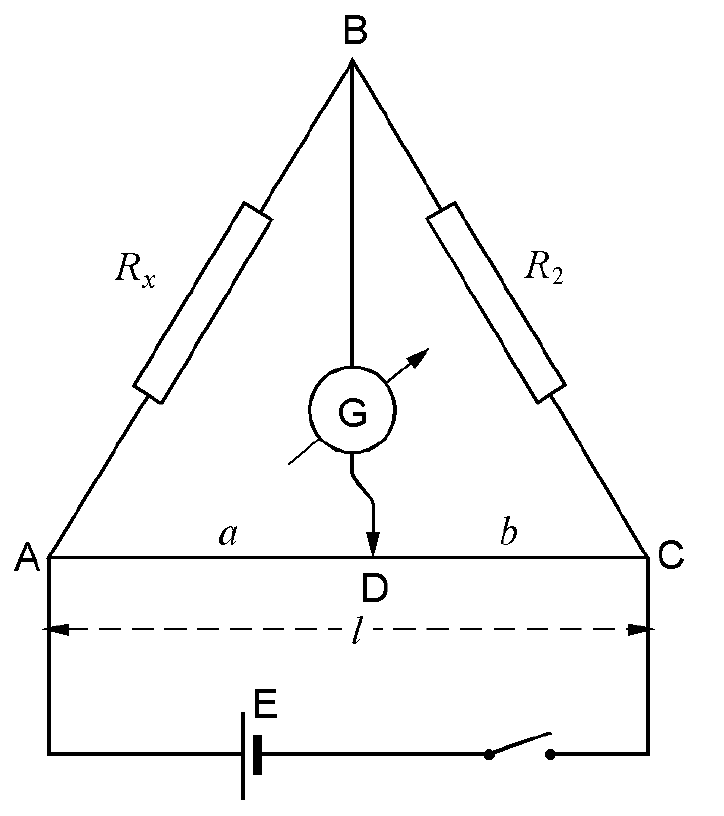
\includegraphics[scale=0.2]{schemat}
		\caption{Schemat elektryczny mostka \\ \textit{Źródło: Pracownia Fizyczna WFiIS AGH - „Ćwiczenie nr 32: Mostek Wheatstone'a”} }
		\label{schematUkladu}
	\end{figure}
	
%--------------------------------------------------------------------------------------------------------------


	\section{Wykonanie ćwiczenia}
	
	\begin{enumerate}
		\item Połączenie układu elektrycznego według schematu
		\item Wykonanie pomiarów wszystkich nieznanych oporników wmontowanych w płytkę z pleksiglasu oraz zapisanie wyników do tabeli
		\item Wykonanie anologicznych pomiarów dla równoległego i szeregowego połączenia oporników oraz zapisanie wyników do tabeli
	\end{enumerate}

%--------------------------------------------------------------------------------------------------------------
	
	\section{Opracowanie danych pomiarowych}
Długość druta oporowego została zmierzona i wynosi $100$ cm. Jest ona dana zmienną $l$
\begin{equation}
l = 100 \textrm{ cm}
\end{equation}
Rezystancja z danych podanych w tabelach zostaje obliczona za pomocą wzoru:
\begin{equation}
R_x = \frac{Ra}{l-a}
\end{equation}
gdzie $R$ to znana oporność, $l$ to długość drutu oporowego i $a$ to zmierzona odległość wysunięcia kontaktu ślizgowego. Krok zmiany znanej rezystancji został dostosowany do danego opornika aby zmiana wychylenia mikroamperomierza była zauważalna.

\subsection{Pomiar dla opornika 1}
W tabeli \ref{tabela:opornik1} zestawiono pomiary przeprowadzone dla opornika 1. Przyjęty został krok zmiany znanej rezystancji $0.5 ~\Omega$.

\begin{table}[!h]
	\centering
	\resizebox{\textwidth}{!}{\begin{tabular}{| c | c | c | c | c | c | c | c | c | c | c |}
			\hline
			Rezystancja opornika znanego $R$ [$\Omega$] & 12.5 & 13.0 & 13.5 & 14.0 & 14.5 & 12.0 & 11.5 & 11 & 10.5 & 10  \\ \hline
			Długość  $a$ [mm] & 500 & 491 & 482 & 473 & 464 & 510 & 519 & 529 & 543 & 555 \\ \hline
			Opór $R_1$ obliczona [$\Omega$] & 12.50 & 12.54 & 12.56 & 12.57 & 12.55 & 12.49 & 12.41 & 12.35 & 12.48 & 12.47 \\ \hline
	\end{tabular}}
	\caption{Wyniki pomiarów dla opornika nr 1}
	\label{tabela:opornik1}
\end{table}

Aby uzyskać rezystancję opornika obliczamy średnią arytmetyczną z wyników z tabeli powyżej:
\begin{equation}
\overline{R_1} = \frac{\sum_{i = 1}^{10} R_{1_i}}{10} \approx 12.49 \textrm{ $\Omega$}
\end{equation}

%----------------------------------------------------------------------------------------------------------	

\subsection{Pomiar dla opornika 2}
W tabeli \ref{tabela:opornik2} zestawiono pomiary przeprowadzone dla opornika 2. Przyjęty został krok zmiany znanej rezystancji $1 ~\Omega$ z wyjątkiem pierwszego pomiaru dla $a = 500$ mm (celem uzyskania wyniku równego rezystancji znanej).

\begin{table}[!h]
	\centering
	\resizebox{\textwidth}{!}{\begin{tabular}{| c | c | c | c | c | c | c | c | c | c | c |}
			\hline
			Rezystancja opornika znanego $R$ [$\Omega$] & 35.8 & 36.0 & 37.0 & 38.0 & 39.0 & 35.0 & 34.0 & 33.0 & 32.0 & 31.0  \\ \hline
			Długość  $a$ [mm] & 500 & 494 & 487 & 480 & 473 & 502 & 509 & 517 & 524 & 533 \\ \hline
			Opór $R_2$ obliczona [$\Omega$] & 35.80 & 35.15 & 35.12 & 35.08 & 35.00 & 35.28 & 35.25 & 35.32 & 35.23 & 35.38 \\ \hline
	\end{tabular}}
	\caption{Wyniki pomiarów dla opornika nr 2}
	\label{tabela:opornik2}
\end{table}

Aby uzyskać rezystancję opornika obliczamy średnią arytmetyczną z wyników z tabeli powyżej:
\begin{equation}
\overline{R_2} = \frac{\sum_{i = 1}^{10} R_{2_i}}{10} \approx 35.26 \textrm{ $\Omega$}
\end{equation}

%----------------------------------------------------------------------------------------------------------
\newpage
\subsection{Pomiar dla opornika 3}
W tabeli \ref{tabela:opornik3} zestawiono pomiary przeprowadzone dla opornika 3. Przyjęty został krok zmiany znanej rezystancji $2 ~\Omega$ z wyjątkiem pierwszego pomiaru dla $a = 500$ mm (celem uzyskania wyniku równego rezystancji znanej).

\begin{table}[!h]
	\centering
	\resizebox{\textwidth}{!}{\begin{tabular}{| c | c | c | c | c | c | c | c | c | c | c |}
			\hline
			Rezystancja opornika znanego $R$ [$\Omega$] & 72.1 & 74.0 & 76.0 & 78.0 & 80.0 & 70.0 & 68.0 & 66.0 & 64.0 & 62.0  \\ \hline
			Długość  $a$ [mm] & 500 & 491 & 481 & 476 & 469 & 506 & 508 & 513 & 520 & 527 \\ \hline
			Opór $R_3$ obliczona [$\Omega$] & 72.10 & 71.38 & 70.44 & 70.85 & 70.66 & 71.70 & 70.21 & 69.52 & 69.33 & 69.08 \\ \hline
	\end{tabular}}
	\caption{Wyniki pomiarów dla opornika nr 3}
	\label{tabela:opornik3}
\end{table}

Aby uzyskać rezystancję opornika obliczamy średnią arytmetyczną z wyników z tabeli powyżej:
\begin{equation}
\overline{R_3} = \frac{\sum_{i = 1}^{10} R_{3_i}}{10} \approx 70.53 \textrm{ $\Omega$}
\end{equation}

%----------------------------------------------------------------------------------------------------------

\subsection{Połączenie szeregowe}
\subsubsection{Obliczenie rezystancji}
W połaczeniu szeregowym opór zastępczy jest równy sumie oporów rezystorów na połączeniu, stąd wynika, że mierzony opór powinien wynosić:
\begin{equation}
R_{s_{obl}} = R_1 + R_2 + R_3 = 118.28~\Omega
\end{equation}

\subsubsection{Pomiar rezystancji}
W tabeli \ref{tabela:szeregowe} zestawiono pomiary przeprowadzone połączenia szeregowego oporników $R_1$, $R_2$, $R_3$. Przyjęty został krok zmiany znanej rezystancji $5 ~\Omega$ z wyjątkiem pierwszego pomiaru dla $a = 500$ mm (celem uzyskania wyniku równego rezystancji znanej).

\begin{table}[!h]
	\centering
	\resizebox{\textwidth}{!}{\begin{tabular}{| c | c | c | c | c | c | c | c | c | c | c |}
			\hline
			Rezystancja opornika znanego $R$ [$\Omega$] & 116.3 & 120.0 & 125.0 & 130.0 & 135.0 & 110.0 & 105.0 & 100.0 & 95.0 & 90  \\ \hline
			Długość  $a$ [mm] & 500 & 496 & 484 & 474 & 465 & 514 & 526 & 538 & 554 & 568 \\ \hline
			Opór $R_{s}$ obliczona [$\Omega$] & 116.30 & 118.10 & 117.25 & 117.15 & 117.34 & 116.34 & 116.52 & 116.45 & 118.00 & 118.33 \\ \hline
	\end{tabular}}
	\caption{Wyniki pomiarów dla połączenia szeregowego}
	\label{tabela:szeregowe}
\end{table}

Aby uzyskać rezystancję opornika obliczamy średnią arytmetyczną z wyników z tabeli powyżej:
\begin{equation}
\overline{R_{s}} = \frac{\sum_{i = 1}^{10} R_{{s}_i}}{10} \approx 117.18 \textrm{ $\Omega$}
\end{equation}

%----------------------------------------------------------------------------------------------------------

\subsection{Połączenie równoległe}
\subsubsection{Obliczenie rezystancji}
W połaczeniu równoległym opór zastępczy jest równy odwrotności sumy odwrotności oporów rezysotrów układu. Wynika stąd, że spodziewana oporność połączenia będzie wynosić:
\begin{equation}
R_{r_{obl}} = \frac{1}{\frac{1}{R_1} + \frac{1}{R_2} + \frac{1}{R_3}} \approx 8.16~\Omega 
\end{equation}

\subsubsection{Pomiar rezystancji}
W tabeli \ref{tabela:rownolegle} zestawiono pomiary przeprowadzone połączenia równoległego oporników $R_1$, $R_2$, $R_3$. Przyjęty został krok zmiany znanej rezystancji $0.5 ~\Omega$ z wyjątkiem pierwszego pomiaru dla $a = 500$ mm (celem uzyskania wyniku równego rezystancji znanej).

\begin{table}[!h]
	\centering
	\resizebox{\textwidth}{!}{\begin{tabular}{| c | c | c | c | c | c | c | c | c | c | c |}
			\hline
			Rezystancja opornika znanego $R$ [$\Omega$] & 8.0 & 8.5 & 9.0 & 9.5 & 10.0 & 7.5 & 7.0 & 6.5 & 6.0 & 5.5  \\ \hline
			Długość  $a$ [mm] & 500 & 485 & 472 & 459 & 450 & 519 & 534 & 552 & 557 & 596 \\ \hline
			Opór $R_{r}$ obliczona [$\Omega$] & 8.0 & 8.0 & 8.05 & 8.06 & 8.18 & 8.09 & 8.02 & 8.01 & 7.95 & 8.11 \\ \hline
	\end{tabular}}
	\caption{Wyniki pomiarów dla połączenia równoległego}
	\label{tabela:rownolegle}
\end{table}

Aby uzyskać rezystancję opornika obliczamy średnią arytmetyczną z wyników z tabeli powyżej:
\begin{equation}
\overline{R_{r}} = \frac{\sum_{i = 1}^{10} R_{{r}_i}}{10} \approx 8.05 \textrm{ $\Omega$}
\end{equation}

%----------------------------------------------------------------------------------------------------------

\subsection{Analiza niepewności}

\subsubsection{Niepewność pomiarowa długości druta oporowego}

Drut oporowy został rozciagnięty nad całą długością przymiaru milimetrowego, dlatego stosujemy niepewność typu B, czyli wartość działki elementarnej:
\begin{equation}
u(l) = 0.1 \textrm{ cm}
\end{equation}

%----------------------------------------------------------------------------------------------------------

\subsubsection{Niepewność pomiarowa opornika o znanej rezystancji}

Oporność rezystora jest ściśle określona oraz możliwa do regulacji pokrętłami na obudowie urządzenia. Niestety, urządzenie nie oferowało żadnej podanej niepewności na tabliczce znamionowej, przez co należy przyjąć, że ustawiona rezystancja nie jest obarczona żadnym błędem. Jest to nieprawdziwe, ponieważ po sprawdzeniu wartości oporu za pomocą multimetru ustawiona wartość odbiegała od rzeczywistej o niestały procent, przez co nie jest możliwe określić dokładnej niepewności pomiarowej znanej rezystancji.

%----------------------------------------------------------------------------------------------------------

\subsubsection{Niepewność mierzonego oporu}

Niepewność mierzonego oporu należy obliczyć zgodnie z prawem przenoszenia niepewności uzależnione od niepewności pomiarowej druta oporowego zgodnie z wzorem:
\begin{equation}
u(R_{{x}_i}) = \left| \frac{dR_{{x}_i}}{da} u(a) \right| = R \frac{l}{(l-a)^2} u(a)
\end{equation}
Powyższy wzór został zastosowany dla każdego pojedynczego pomiaru każdego opornika/zestawu oporników a z otrzymanych wyników została obliczona średnia arytmetyczna stanowiąca finalny wynik niepewności pomiarowej mierzonego oporu. Zatem wzór końcowy niepewności określony jest równaniem:
\begin{equation}
u(R_x) = \frac{\sum_{i = 1}^{10} R_{{x}_i}}{10}
\end{equation}
Niepewność wynosi odpowiednio dla poszczególnych rezystorów:
\begin{itemize}
	\item Opornik 1
	\begin{equation}
	u(R_1) = 0.05~\Omega
	\end{equation}
	
	\item Opornik 2
	\begin{equation}
	u(R_2) = 0.14~\Omega
	\end{equation}
	
	\item Opornik 3
	\begin{equation}
	u(R_3) = 0.28~\Omega
	\end{equation}
	
	\item Połaczenie szeregowe
	\begin{equation}
	u(R_s) = 0.47~\Omega
	\end{equation}
	
	\item Połaczenie równoległe
	\begin{equation}
	u(R_r) = 0.03~\Omega
	\end{equation}
\end{itemize}

\subsubsection{Niepewność złożona obliczonej rezystancji}
Niepewność obliczenia rezystancji jest niepewnością złożoną uzależnioną od niepewności pomiaru oporności $R_1$, $R_2$ oraz $R_3$ i wyraża się ją wzorem:
\begin{equation}
u(R) = \sqrt{\left( \frac{\delta R}{\delta R_1} \right)^2 u(R_1)^2 + \left( \frac{\delta R}{\delta R_2} \right)^2 u(R_2)^2 + \left( \frac{\delta R}{\delta R_3} \right)^2 u(R_3)^2}
\label{niepewnosc_zlozona}
\end{equation}
Stąd dla połączenia szeregowego uzyskujemy niepewność określoną wzorem:
\begin{equation}
u(R_{s_{obl}}) = \sqrt{u(R_1)^2 + u(R_2)^2 + u(R_3)^2} \approx 0.32~\Omega
\end{equation}
Dla połączenia równoległego niepewność złożona, po podstawieniu do wzoru \ref{niepewnosc_zlozona}, wynosi:
\begin{equation}
u(R_{r_{obl}}) \approx 0.02~\Omega
\end{equation}
%--------------------------------------------------------------------------------------------------------------


\section{Podsumowanie}
Wyniki z uwzględnieniem niepewności pomiarowych zostały przedstawione w tabeli poniżej. Dla oporników 1, 2 oraz 3 wartość rezystancji jest wyznaczana tylko doświadczalnie.
\begin{table}[!h]
	\centering
	\begin{tabular}{| c | c | c |}
		\cline{1-2}
		\textbf{Opornik} & \textbf{Oporność wyznaczona [$\Omega$]} \\ \cline{1-2}
		Opornik 1 & $12.49 \pm 0.05$ \\ \cline{1-2}
		Opornik 2 & $35.26 \pm 0.14$ \\ \hline
		Opornik 3 & $70.53 \pm 0.28$ & \textbf{Oporność obliczona [$\Omega$]} \\ \hline
		Połączenie szeregowe & $117.18 \pm 0.47$ & $118.28 \pm 0.32$\\ \hline
		Połączenie równoległe & $8.05 \pm 0.03$ & $8.16 \pm 0.02$\\ \hline
	\end{tabular}
	\caption{Podsumowanie wyników doświadczenia wraz z niepewnościami}
\end{table}

%--------------------------------------------------------------------------------------------------------------

\section{Wnioski}

Wykonanie tego ćwiczenia pozwoliło nam zrozumieć prawa Kirchhoffa oraz zależności określające opór dla połączeń szeregowych oraz równoległych ze strony praktycznej. W ciekawy sposób mogliśmy na nowo nauczyć się czegoś, co znaliśmy wyłącznie z książek. Wyniki przedstawione w tabeli 6 wskazują na to, że udało nam się wykonać doświadczenie poprawnie. Różnice między wartościami wyznaczonymi a obliczonymi wynikają z niedokładnością przyrządów pomiarowych (t.j. niedokładne wyznaczanie wartości przez opornicę dekadową, kontakt ślizgowy, który utrudniał dokładny odczyt wartości $a$ i $b$) oraz czynnika ludzkiego. Wadliwość elementów układu znacząco wpłynęła na wyniki końcowe. Mimo niedokładności przyrządów uzyskane wyniki nie pokrywają się z wyznaczonymi w stu procentach, jednak mieszczą się w zadawalającym przedziale. 

\end{document}